\section{Character and Enemy Sheets}

\subsection{General information}
\begin{itemize}
	\item One turn equals to three seconds of real-time gameplay.
	\item In each turn a character can move maximum by its movement value (in meters) and can perform maximum one action from the list in its sheet.
	\item Although the attacks of every character corresponds to a weapon or a spell present in the GDD, ranges have been adapted to Elby's skills range
	\item Both characters and monsters have a cooldown linked to individual skills. The minimum value of the cooldown is one turn (three seconds of real time game play) and is applied for the basic skills of the characters. The more powerful the skill the greater the cooldown will be.
	\item Technical abbreviations:
	\begin{itemize}
		\item \textbf{AC} Armor Class, the higher is this value, the easier is to hit the character.
		\item \textbf{HP} Hit Points, the maximum amount of damage a character can take before being defeated.
		\item \textbf{NRG} Energy points required for Elby's Active Skills.
		\item \textbf{THAC0} To Hit Armor Class 0, the roll with a d20 a character needs to hit a enemy with an AC value of 0.
		\item \textbf{d4} a dice with 4 sides.
		\item \textbf{d6} a dice with 6 sides.
		\item \textbf{d8} a dice with 8 sides.
		\item \textbf{d20} a dice with 20 sides.
	\end{itemize}
\end{itemize}

\newpage

\subsection{Bad Eleven}

\begin{figure}[H]
	\centering
	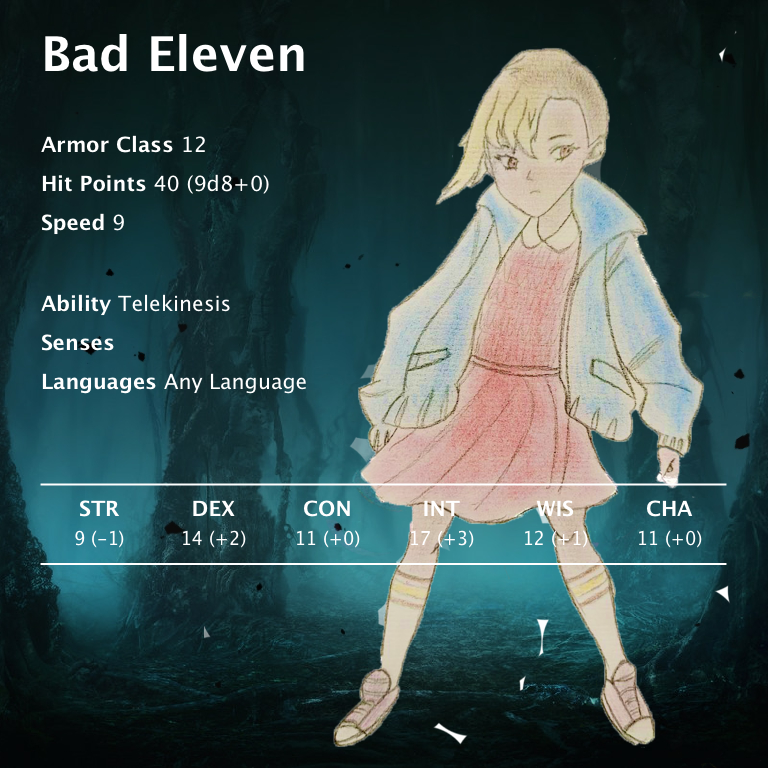
\includegraphics[width=0.8\linewidth]{images/visual_stats/badeleven.png}
\end{figure}

\vspace*{2mm}

\begin{center}
	\begin{tabular}[c]{| p{2cm} | p{2,5cm} | p{1,7cm} | p{1,7cm} | p{2cm} | p{3,5cm} | }
		\hline
		\textbf{Skill} & \textbf{Damage} & \textbf{Range} & \textbf{Target} & \textbf{Energy} & \textbf{D\&D Ref}\\
		\hline
		Psyhit & 2d4 (avg 5) & 2m & 1 & -1 NRG & Magic missile (Lv. 1)\\
		\hline
		Psychain & 1d4 (avg 2,5) & 2m & 1 & -5 NRG & Web (Lv. 2)\\
		\hline
		Psypush & 1d4 (avg 2,5) & 2m & 1 & -10 NRG & Thunderwave (Lv. 1)\\
		\hline
		Psyslash & 2d6 (avg 7) & 3m & Front & -15 NRG & Airslash (Lv. 5)\\
		\hline
		Psyarrow & 4d6 (avg 14) & 5m & 1 (pierce) & -25 NRG & Fireball (Lv. 3)\\
		\hline
		Psyburst & 3d8 (avg 13,5) & 6m (aoe) & - & -20 NRG & Explosion (Lv. 8)\\
		\hline
		Psyshield & - & 0m & Self & -10 NRG & Prismatic wall (Lv. 9)\\
		\hline
		Mastermind & - & 0m & Self & +4 NRG (per turn for 5 turns) & Prestidigitation (Lv. 0)\\
		\hline
		Focus & - & 0m & Self & +10 NRG & Spell focus (Lv. 0)\\
		\hline
	\end{tabular}
\end{center}


\subsection{Enemies}

\subsubsection{Demobat}
\vspace*{0.3cm}
\begin{figure}[H]
	\centering
	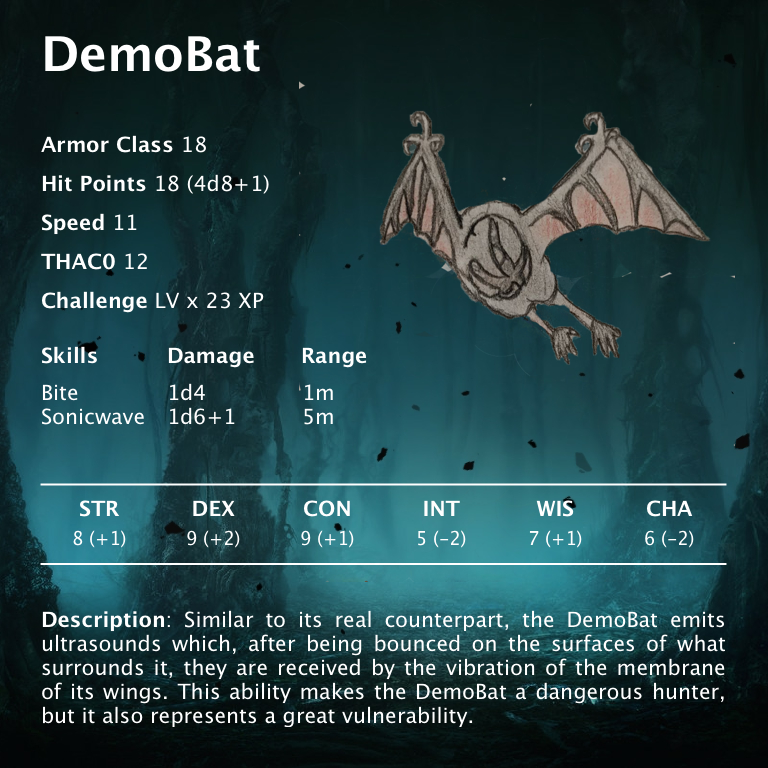
\includegraphics[width=0.9\linewidth]{images/visual_stats/demobat.png}
\end{figure}
\newpage
\begin{figure}[H]
	\centering
	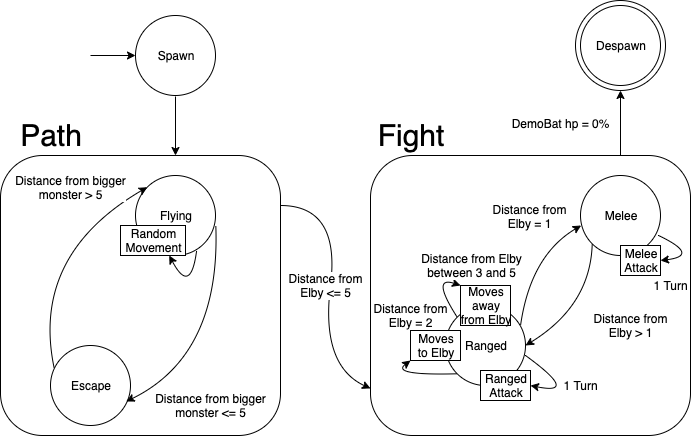
\includegraphics[width=0.8\linewidth]{images/graphs/fsa/fsa_demobat.png}
\end{figure}
\vspace*{4mm}
\textbf{Damage taken - Elby vs 1 Demobat}\\
\newline
$\star$ Using only bite\\
$12-7 = (THACO\:Demobat) - (AC\:Elby) = 5$\\
$(20-5)/20 = 3/4 = 0,75$\\
$0,75 * (1d4 = 2,5) = 1,875$ damage per turn\\
$40 HP/ 1,875 = 21,33$ turns (after 22 turns Elby dies)\\
\newline
$\star$ Using only sonicwave\\
$12-7 = (THACO\:Demobat) - (AC\:Elby) = 5$\\
$(20-5)/20 = 3/4 = 0,75$\\
$0,75 * (1d6+1 = 4,5) = 3,375$ damage per turn\\
$40 HP/ 3,375 = 11,85$ turns (after 12 turns Elby dies)\\


\textbf{Damage dealt - Elby vs 1 Demobat}\\
\newline
$\star$ Using only Psyslash\\
$10-10 = (THACO\:Elby) - (AC\:Demobat) = 0$\\
$(20-0)/20 = 1$ \\
$1 * (2d6 = 7) = 7$ damage per turn\\
$18/ 7 =2,5$ (after 3 turns Elby wins)\\
\newline
$\star$ With Psyarrow\\
$10-10 = (THACO\:Elby) - (AC\:Demobat) = 0$\\
$(20-0)/20 = 1$ \\
$1 * (2d6 = 7) * 2/3  = 7 * 2/3 = 4,6$ damage per turn of Psyslash\\
$1 * (4d6 = 4,6) * 1/3 = 14 * 1/3  = 4,6$ damage per turn of Psyarrow\\
$4,6*2= 9,2$ per turn\\
$18 / 9,2 = 1,95$ (after 2 turns Elby wins)\\
\newpage

\subsubsection{Demomole}
\vspace*{0.3cm}
\begin{figure}[H]
	\centering
	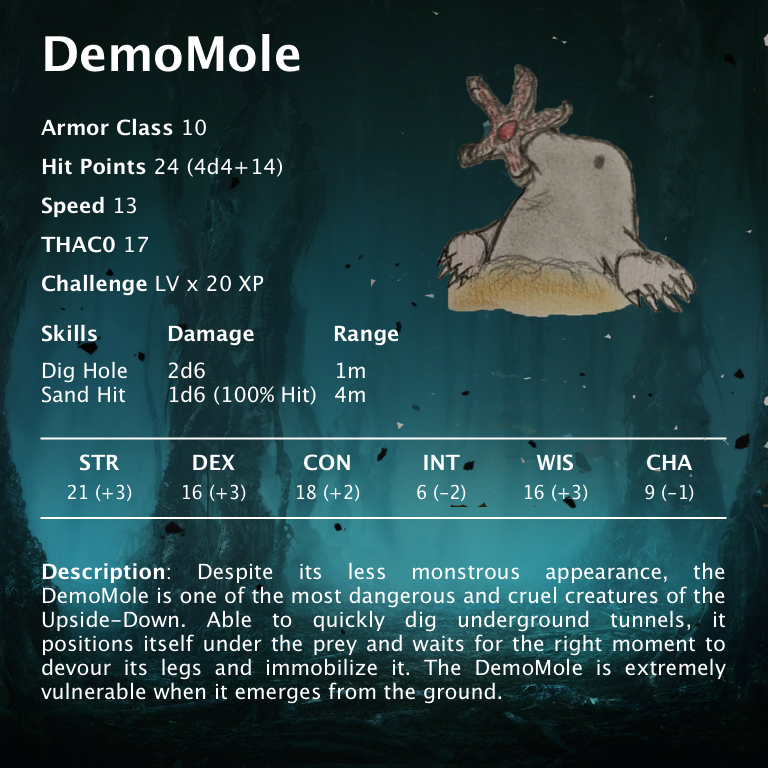
\includegraphics[width=0.9\linewidth]{images/visual_stats/demomole.png}
\end{figure}
\newpage
\begin{figure}[H]
	\centering
	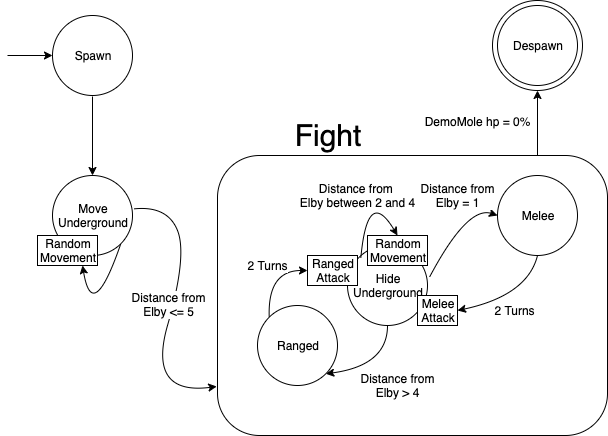
\includegraphics[width=0.8\linewidth]{images/graphs/fsa/fsa_demomole.png}
\end{figure}
\vspace*{4mm}
\textbf{Damage taken - Elby vs 1 Demomole}\\
\newline
$\star$ Using only sand hit\\
$17-7 = (THACO\:Demomole) - (AC\:Elby) = 10$\\
$(20-10)/20 = 1/2 = 0,5$\\
$0,5 * (2d6 = 7) = 3,5$ damage per turn\\
$40 HP / 3,5 = 11,42$ turns (after 12 turns Elby dies)\\
\newline
$\star$ Using only dig hole \\
This attack can’t fail!\\
$1*(1d6 = 3,5) = 3,5$ damage per turn\\
$40 / 3,5 = 11,42$ turns (after 12 turns Elby dies)\\

\textbf{Damage dealt - Elby vs 1 Demomole}\\
\newline
$\star$ Using only Psyslash\\
$10-10 = (THACO\:Elby) - (AC\:Demomole) = 0$\\
$(20-0)/20 = 20/20 = 1$\\
$1 * (2d6 = 7) = 7\:damage\:per\:turn$\\
$24 / 7 = 3,42$ (after 4 turns Elby wins)\\
\newline
$\star$ With Psyarrow\\
$10-10 = (THACO\:Elby) - (AC\:Demomole) = 0$\\
$(20-0)/20 = 20/20 = 1$\\
$1 * (2d6 = 7) * 2/3  = 5,25 * 2/3 = 4,6$ damage per turn of Psyslash\\
$1 * (4d6 = 14) * 1/3 = 10,5 * 1/3 = 4,6$ damage per turn of Psyarrow\\
$4,6 * 2 = 9,2$ per turn\\
$24 / 9,2 = 2,6$ (after 3 turns Elby wins)\\
\newpage


\subsubsection{Demorat}
\vspace*{0.3cm}
\begin{figure}[H]
	\centering
	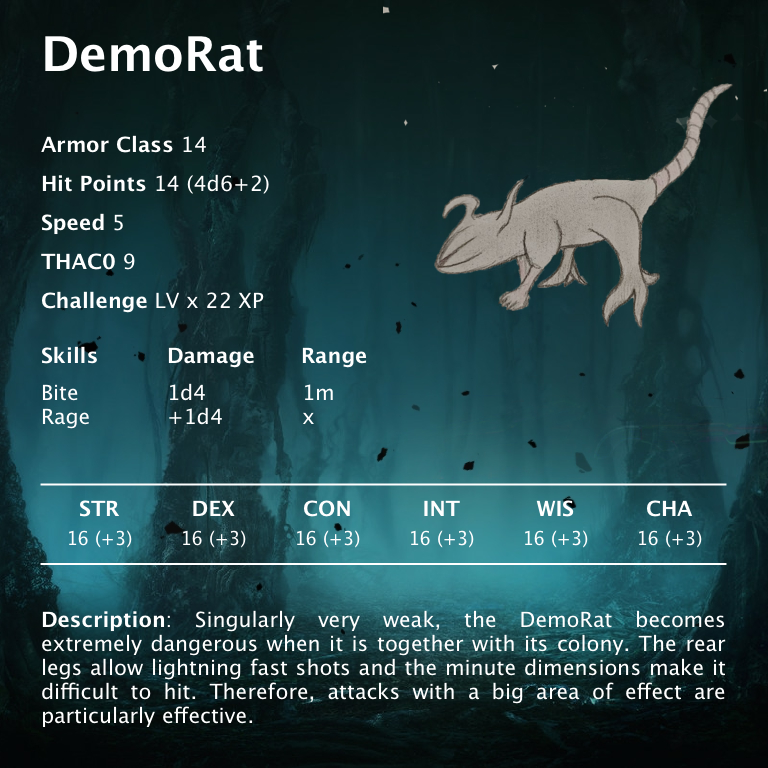
\includegraphics[width=0.9\linewidth]{images/visual_stats/demorat.png}
\end{figure}
\newpage
\begin{figure}[H]
	\centering
	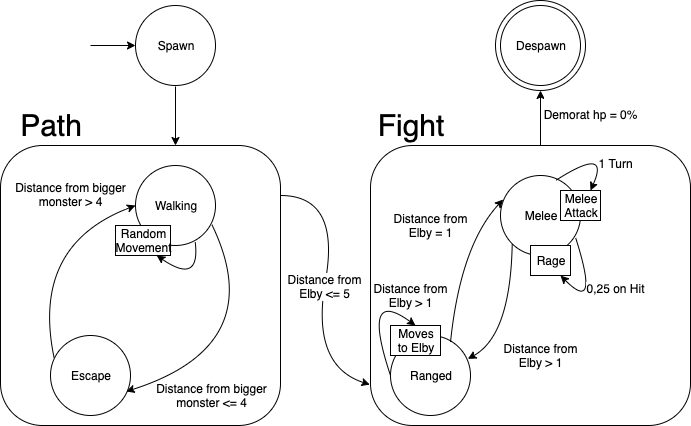
\includegraphics[width=0.8\linewidth]{images/graphs/fsa/fsa_demorat.png}
\end{figure}
\vspace*{4mm}
\textbf{Damage taken - Elby vs 1 Demorat}\\
\newline
$\star$ Using only bite\\
$9-7 = (THACO\:Demorat) - (AC\:Elby) = 2$\\
$(20-2)/20 =9/10 = 0,9$\\
$0,9 * (1d4 = 2,5) = 2,25$ damage per turn\\
$40 HP/ 2,25 = 17,78$ (after 18 turns Elby dies)\\


\textbf{Damage dealt - Elby vs 1 Demorat}\\
\newline
$\star$ Using only Psyslash\\
$10-10 = (THACO\:Elby) - (AC\:Demorat) = 0$\\
$(20-0)/20 = 1$ \\
$1 * (2d6 = 7) = 7$ damage per turn\\
$14/ 7 = 2$ (after 2 turns Elby wins)\\
\newline
$\star$ With Psyarrow\\
$10-10 = (THACO\:Elby) - (AC\:Demorat) = 0$\\
$(20-0)/20 = 1$\\
$1 * (2d6 = 7) * 2/3 = 7 * 2/3 = 4,6$ damage per turn of Psyslash\\
$1 * (4d6 = 14) * 1/3 = 14 * 1/3 = 4,6$ damage per turn of Psyarrow\\
$4,6*2= 9,2$ per turn\\
$14 / 9,2 = 1,52$ (after 2 turns Elby wins)\\

\newpage


\subsubsection{Demodog}
\vspace*{0.3cm}
\begin{figure}[H]
	\centering
	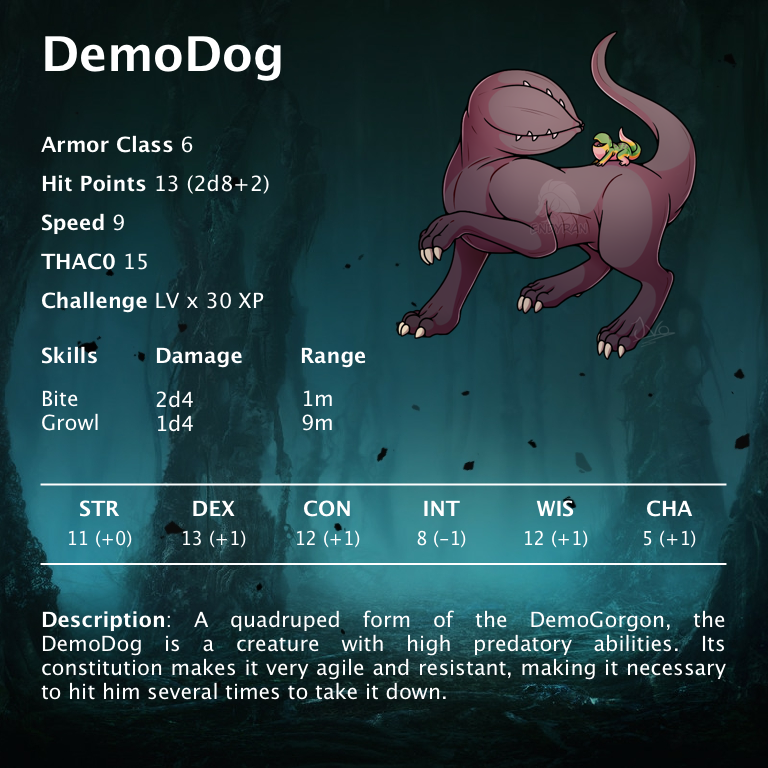
\includegraphics[width=0.9\linewidth]{images/visual_stats/demodog.png}
\end{figure}
\newpage
\begin{figure}[H]
	\centering
	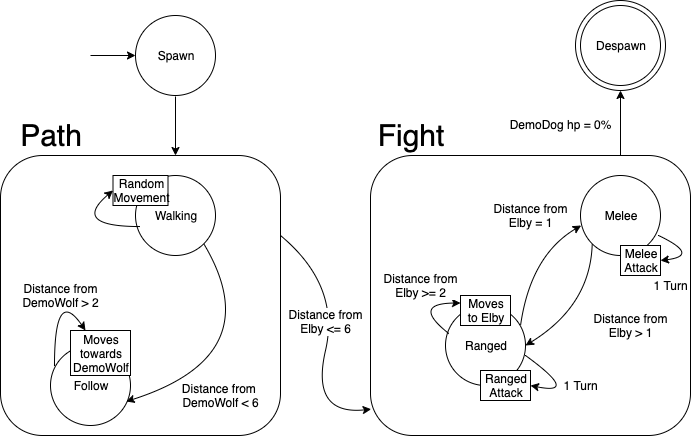
\includegraphics[width=0.8\linewidth]{images/graphs/fsa/fsa_demodog.png}
\end{figure}
\vspace*{4mm}
\textbf{Damage taken - Elby vs 1 Demodog}\\
\newline
$\star$ Using only bite\\
$15-7 = (THACO\:Demodog) - (AC\:Elby) = 8$\\
$(20-8)/20 = 12/20 = 3/5 =  0,6$\\
$0,6 * (2d4 = 5) = 3$ damage per turn\\
$40 / 3 = 13,3$ turns (after 14 turns Elby dies)\\
\newline
$\star$ Using only growl\\
$15-7 = (THACO\:Demodog) - (AC\:Elby) = 8$\\
$(20-8)/20 = 12/20 = 3/5 =  0,6$\\
$0,6 * (1d4 = 2,5) = 1,5$ damage per turn\\
$40 / 1,5 = 26,6$ turns (after 27 turns Elby dies)\\


\textbf{Damage dealt - Elby vs 1 Demodog}\\
\newline
$\star$ Using only Psyslash\\
$10-6 = (THACO\:Elby) - (AC\:Demodog) = 4$\\
$(20-4)/20 = 16/20 = 0,8$\\
$0,8 * (2d6 = 7) = 5,6$ damage per turn\\
$13 / 5,6 = 2,3$ (after 3 turns Elby wins)\\
\newline
$\star$ With Psyarrow\\
$10-10 = (THACO\:Elby) - (AC\:Demodog) = 0$\\
$(20-4)/20 = 16/20 = 0,8$\\
$0,8 * (2d6 = 7) * 2/3  = 5,6 * 2/3 = 3,7$ damage per turn of Psyslash\\
$0,8 * (4d6 = 14) * 1/3 = 11,2 * 1/3 = 3,7$ damage per turn of Psyarrow\\
$3,7 * 2= 7,4$ per turn\\
$13 / 7,4 = 1,75$ (after 2 turns elby wins)\\
\newpage


\subsubsection{Demowolf}
\vspace*{0.3cm}
\begin{figure}[H]
	\centering
	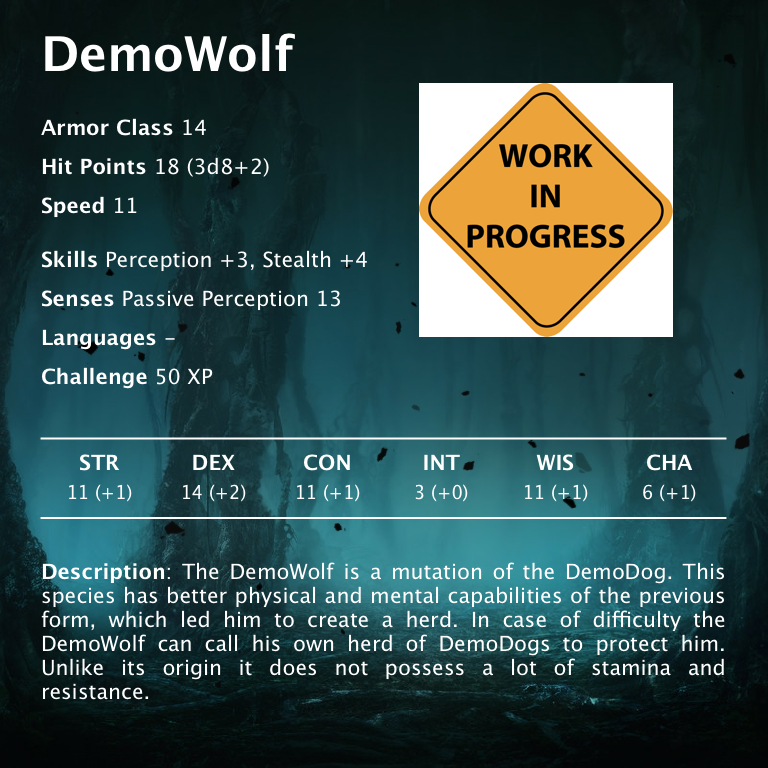
\includegraphics[width=0.9\linewidth]{images/visual_stats/demowolf.png}
\end{figure}
\newpage
\begin{figure}[H]
	\centering
	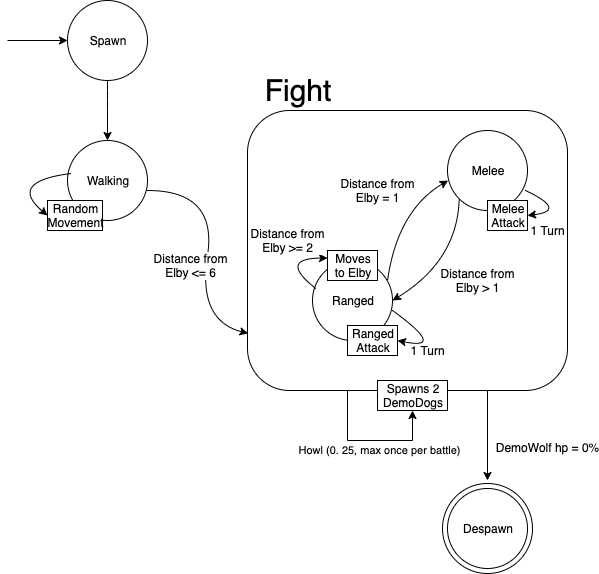
\includegraphics[width=0.7\linewidth]{images/graphs/fsa/fsa_demowolf.png}
\end{figure}
\vspace*{4mm}
\textbf{Damage taken - Elby vs 1 Demowolf}\\
\newline
$\star$ Using only bite\\
$12-7 = (THACO\:Demowolf) - (AC\:Elby) = 5$\\
$(20-5)/20 = 3/4 = 0,75$\\
$0,75 * (2d4+2 = 2,5) = 7$ damage per turn\\
$40 HP / 7 = 5,7$ turns (after 6 turns Elby dies)\\
\newline
$\star$ With growl (summon only one time the Demodogs)\\
$12-7 = (THACO\:Demowolf) - (AC\:Elby) = 5$\\
$(20-5)/20 = 3/4 = 0,75$\\
$0,75 * (2*2d4 =10) = 7,5$ damage per turn\\
$40 HP / 7,5 = 5,3$ turns (after 6 turns Elby dies)\\


\textbf{Damage dealt - Elby vs 1 Demowolf}\\
\newline
$\star$ Using only Psyslash\\
$10-6 = (THACO\:Elby) - (AC\:Demowolf) = 4$\\
$(20-4)/20 = 16/20 = 0,75$\\
$0,75 * (2d6 = 7) = 5,25$ damage per turn\\
$17 / 5,25 = 3,23$ (after 4 turns Elby wins)\\
\newline
$\star$ With Psyarrow\\
$10-5 = (THACO\:Elby) - (AC\:Demowolf) = 5$\\
$(20-5)/20 = 15/20 = 0,75$\\
$0,75 * (2d6 = 7) * 2/3  = 5,25 * 2/3 = 3,5$ damage per turn of Psyslash\\
$0,75 * (4d6 = 14) * 1/3 = 10,5 * 1/3 = 3,5$ damage per turn of Psyarrow\\
$3,5 * 2= 7$ per turn\\
$17 / 7 = 2,42$ (after 3 turns Elby wins)\\
\newpage




\subsubsection{Democerberus}
\vspace*{0.3cm}
\begin{figure}[H]
	\centering
	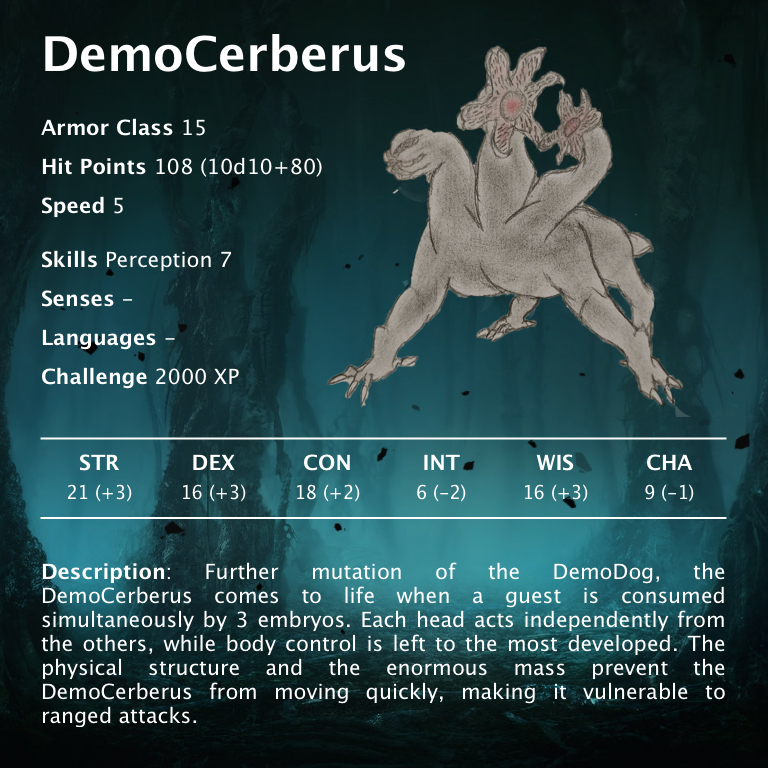
\includegraphics[width=0.9\linewidth]{images/visual_stats/democerberus.png}
\end{figure}
\newpage
\begin{figure}[H]
	\centering
	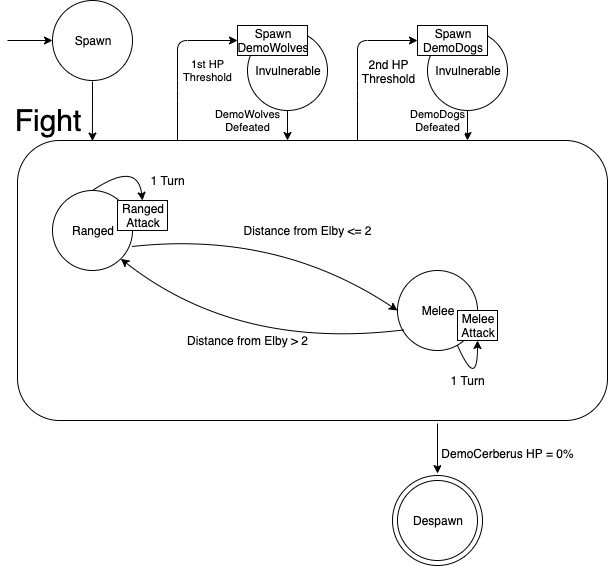
\includegraphics[width=0.9\linewidth]{images/graphs/fsa/fsa_democerberus.png}
\end{figure}

For the battle details see chapter 15 (Fight Outcomes).
\newpage



\subsubsection{NeoDemogorgon}
\vspace*{0.3cm}
\begin{figure}[H]
	\centering
	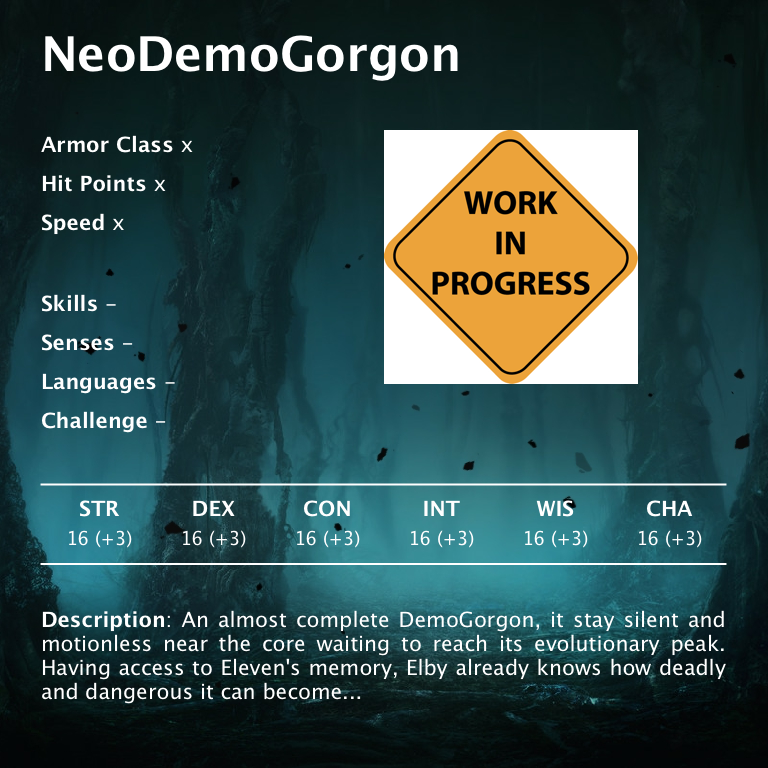
\includegraphics[width=0.9\linewidth]{images/visual_stats/neodemogorgon.png}
\end{figure}
\newpage
\begin{figure}[H]
	\centering
	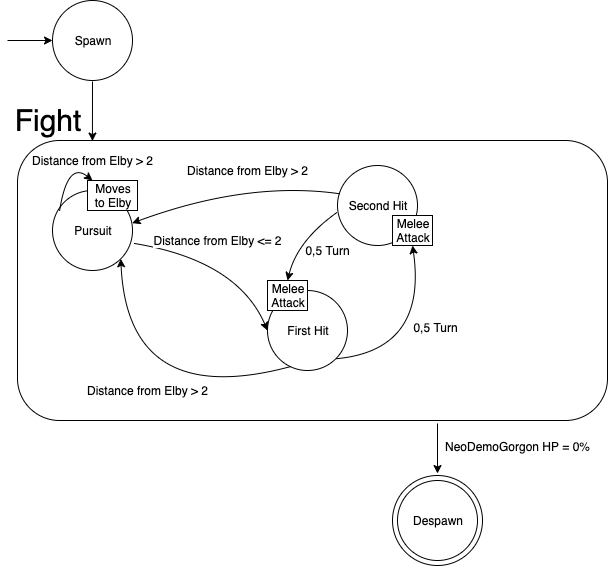
\includegraphics[width=0.8\linewidth]{images/graphs/fsa/fsa_neodemogorgon.png}
\end{figure}


\vspace*{4mm}
\textbf{Damage taken - Elby vs Neodemogorgon}\\
\newline
$10-11 = (THACO\:Elby)-(AC\:Neodemogorgon) = 0$\\
$(20-0)/20 = 1$ (Probability to hit)\\
$1*(4d6=14) = 14$\\
$1*(3d8=13,5) = 13,5$\\
$1*(2d6=7) = 7$\\
$Passive = 3$\\
$(14+7+13,5+3)/3 = 12,5$ each turn\\
$70/12,5 = 5,6$ (after 6 turns elby wins without using Shields)\\

\textbf{Damage dealt - Elby vs Neodemogorgon}\\
\newline
$10-7 = (THACO\:Neodemogorgon)-(AC\:Elby) = 3$\\
$(20-3)/20 = 17/20$ (Probability to hit)\\
$0,85*(3d4=7,5) = 6,375$\\
$0,85*(2d4=5) = 4,25$\\
$6,375+4,25 = 10,625$ each turn\\
$40/10,625 = 3,764$ (after 4 turns elby dies)\\

\newpage


\subsubsection{\#001}
\vspace*{0.3cm}
\begin{figure}[H]
	\centering
	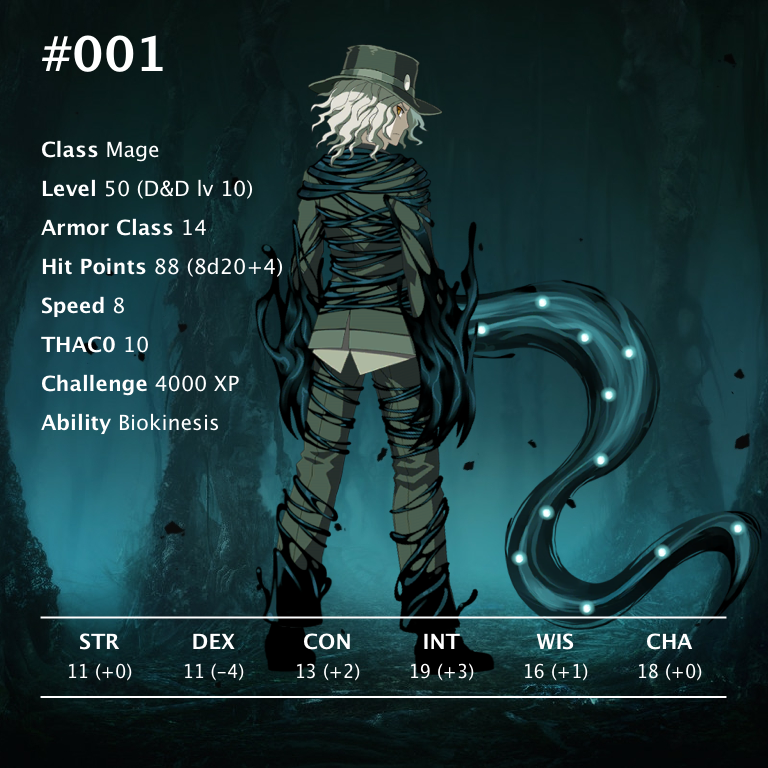
\includegraphics[width=0.9\linewidth]{images/visual_stats/001.png}
\end{figure}
\vspace*{4mm}

\begin{center}
	\begin{tabular}[c]{| p{2,5cm} | p{3,5cm} | p{2cm} | p{2cm} | p{2,8cm} | }
		\hline
		\textbf{Skill} & \textbf{Damage} & \textbf{Range} & \textbf{Target} & \textbf{D\&D Ref}\\
		\hline
		Biospears & 1d10*(3/2) (avg 8,25) & 5m & 1 & Pillar (Lv. 5)\\
		\hline
		Biovenom spit & 8d6*(1/3) (avg 18,6) & 5m & 1 & Fireball (Lv. 3)\\
		\hline
		Bioheal & Restore 6d8 HP (avg 27) & 0m & Self & Wish (Lv. 9)\\
		\hline
		Biospikes ring & 5d6 (avg 17,5) & 3m (aoe) & Self & Ice wall (Lv. 7)\\
		\hline
	\end{tabular}
\end{center}
\newpage


\begin{figure}[H]
	\centering
	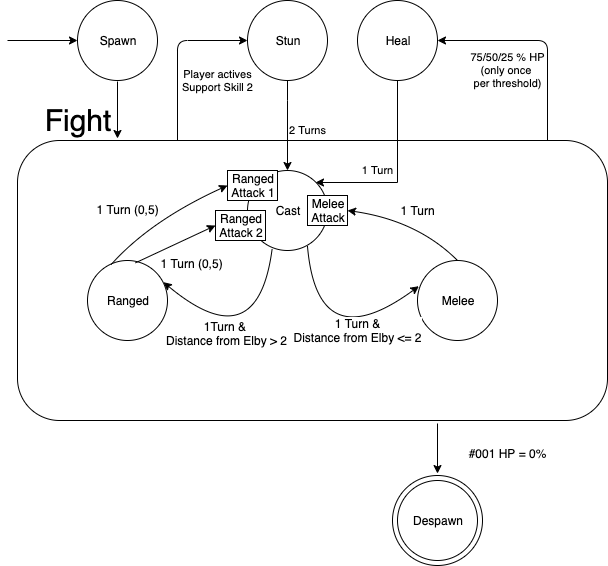
\includegraphics[width=0.9\linewidth]{images/graphs/fsa/fsa_001.png}
\end{figure}

For the battle details see chapter 15 (Fight Outcomes).
\newpage






%\begin{figure}[H]
	%\centering
	%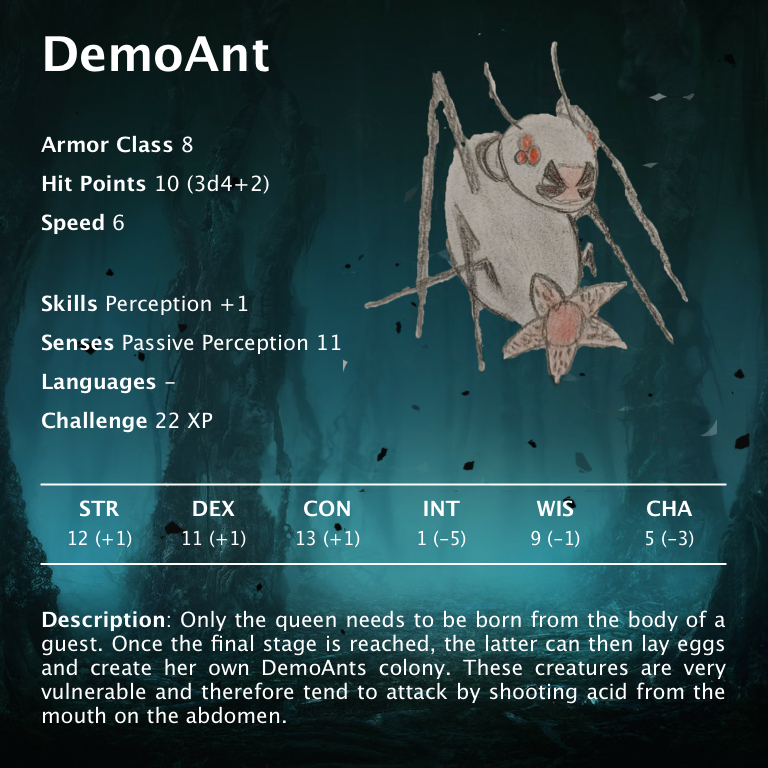
\includegraphics[width=0.7\linewidth]{images/visual_stats/demoant.png}
%\end{figure}


%\begin{figure}[H]
	%\centering
	%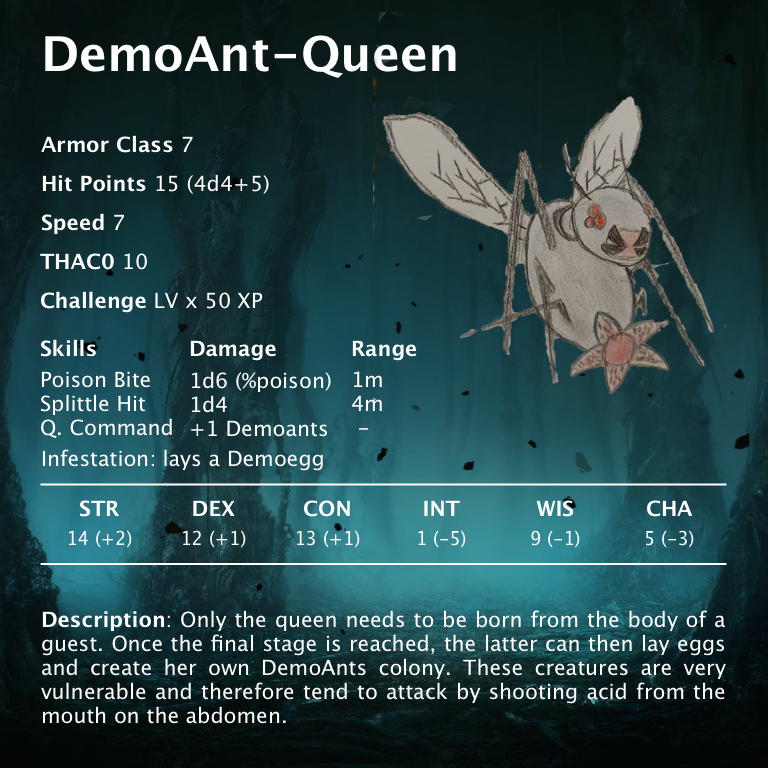
\includegraphics[width=0.7\linewidth]{images/visual_stats/demoant-queen.png}
%\end{figure}


%\begin{figure}[H]
	%\centering
	%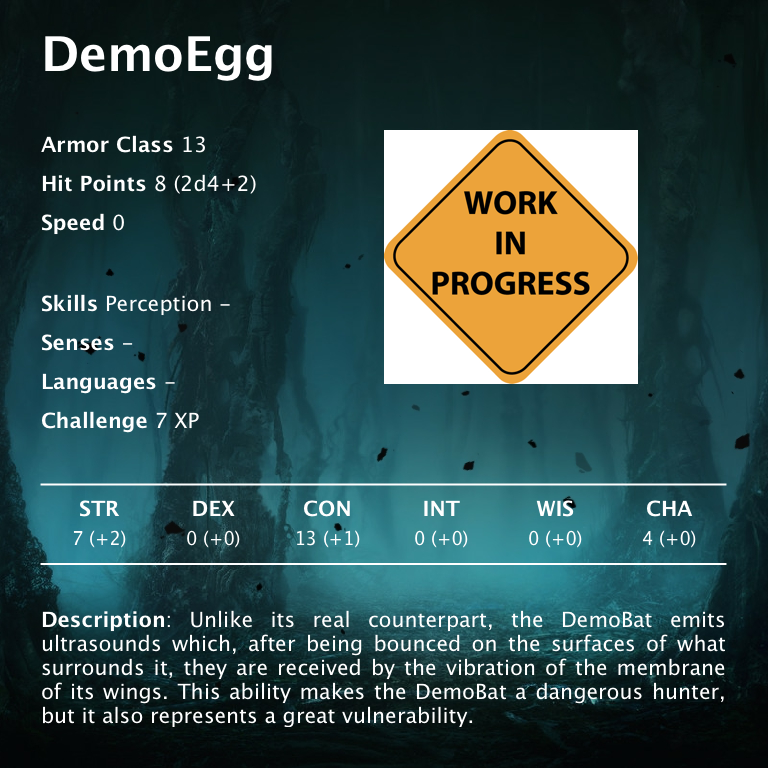
\includegraphics[width=0.7\linewidth]{images/visual_stats/demoegg.png}
%\end{figure}

